\section{Risultati sperimentali}
\label{sec:risult-sper}

In questa sezione verranno discussi i risultati sperimentali dei vari laboratori. Per confrontare le diverse funzioni di reperimento la configurazione di parametri per \textsc{bm25} \`e fissata a quella riportata in tabella \ref{tab:es}, cio\`e $k_1 = 0.0253, b = 0.0221$, per ogni diverso laboratorio. Il risultato del reperimento con il laboratorio 3 che utilizza tale configurazione \`e la \textsc{baseline}.
\`E interessante notare che con l'ottimizzazione i valori trovati per $k_1, b$ sono molto lontani dai valori noti in letteratura. Tali valori (molto vicini a zero) rendono il secondo termine della funzione di reperimento di \textsc{bm25}, 
\[\frac{(k_1 + 1)f_i}{k_1(1-b+b \cdot \frac{dl}{avdl})+f_i},\] 
tendente a $1$. Ci\`o significa che nel nostro contesto, la normalizzazione basata sulle lunghezze del documento non \`e efficace, e inoltre che frequenze diverse di occorrenza dei termini portano a contributi nella funzione di reperimento molto simili. Tale fenomeno pu\`o essere giustificato con il fatto che la maggior parte dei nostri documenti contiene molto pochi termini (solo i titoli), quindi la frequenza dei termini \`e molto meno importante rispetto alla loro presenza. Infatti anche per frequenze molto basse il contributo di questo termine \`e vicino a 1.

Figura \ref{fig:map_all} mostra l'andamento della MAP per le varie funzioni di reperimento, al variare di alcuni parametri della funzione di reperimento.
\begin{figure*}
	\centering
	\begin{subfigure}[htpb]{0.475\textwidth}
		\centering
		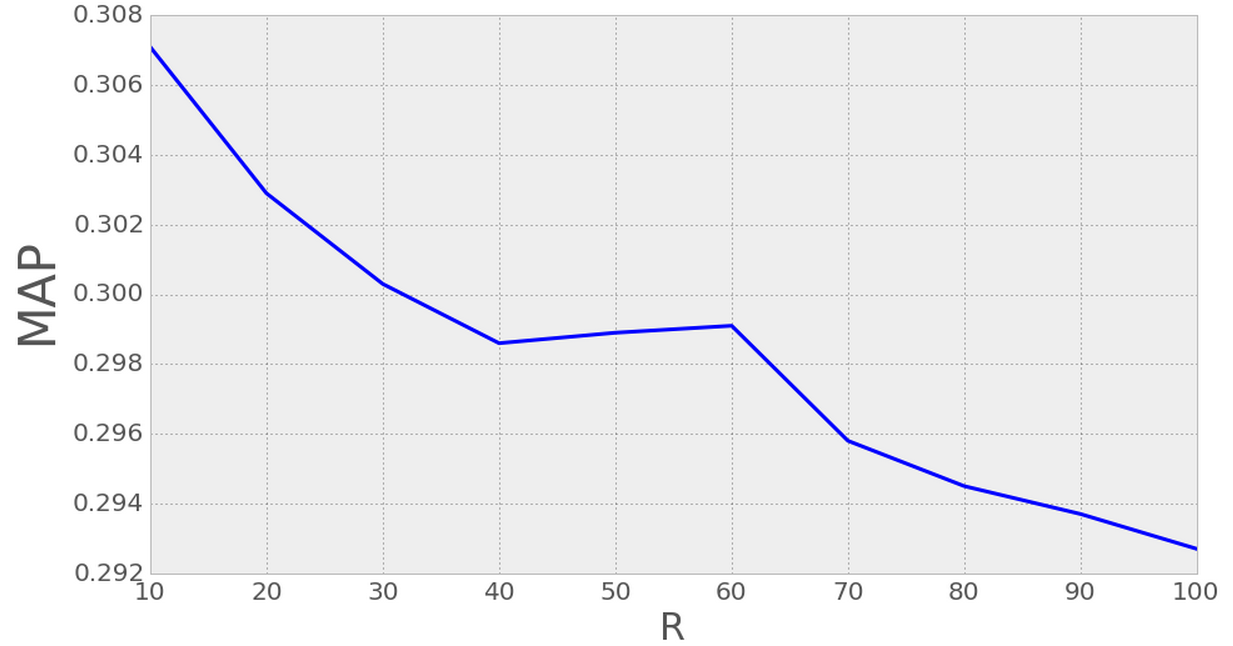
\includegraphics[width=\textwidth]{figures/lab4_R.png}
		\caption[Network2]%
		{{\small Laboratorio 4 (\textsc{rf pseudo}), al variare di $R$.}}    
		\label{fig:lab4_R}
	\end{subfigure}
	\hfill
	\begin{subfigure}[htpb]{0.475\textwidth}  
		\centering 
		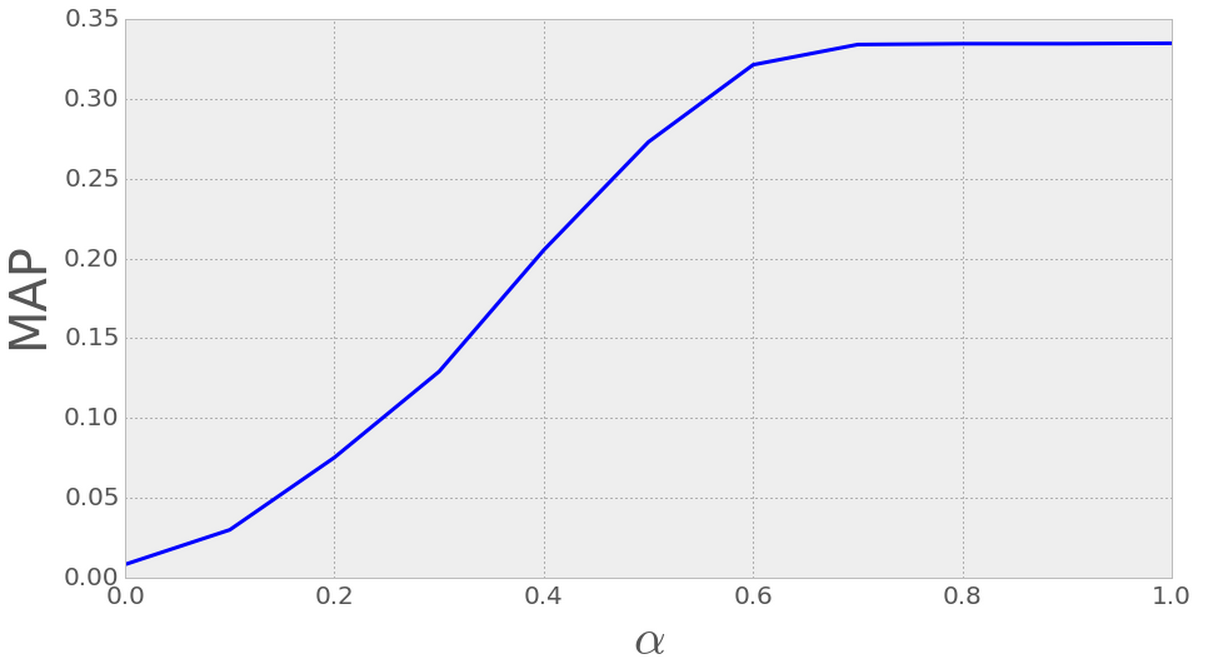
\includegraphics[width=\textwidth]{figures/lab5_alpha.png}
		\caption[]%
		{{\small Laboratorio 5 (\textsc{pagerank}), al variare di $\alpha$.}}    
		\label{fig:lab5_a}
	\end{subfigure}
	\vskip\baselineskip
	\begin{subfigure}[htpb]{0.475\textwidth}   
		\centering 
		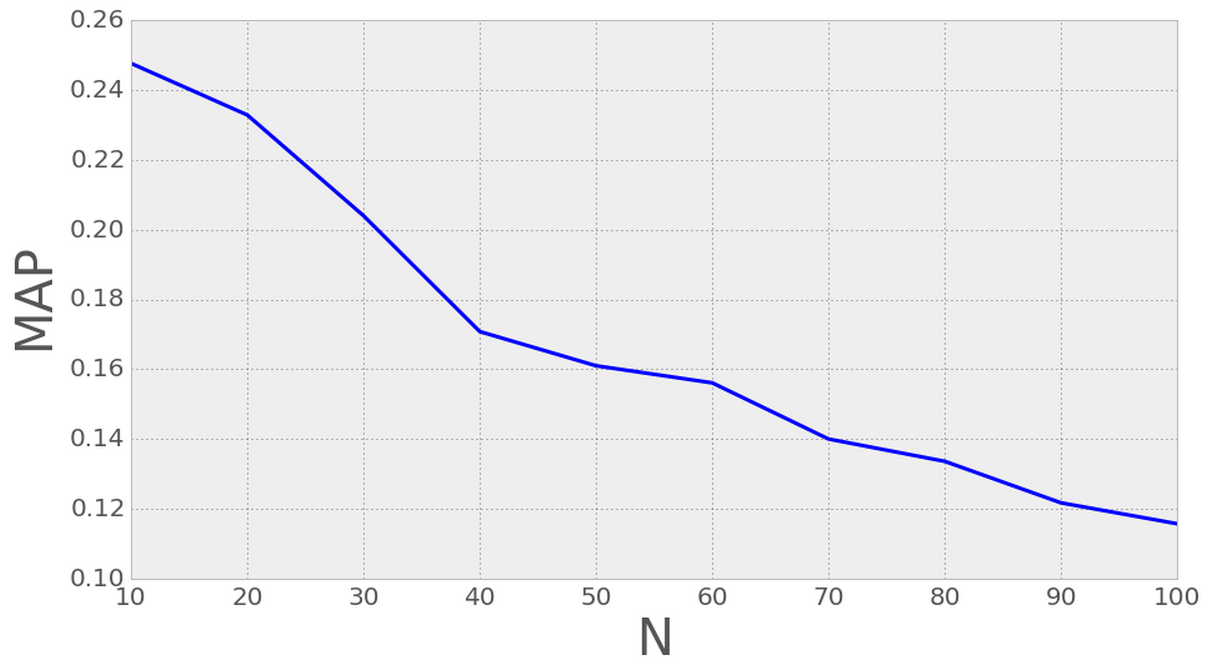
\includegraphics[width=\textwidth]{figures/lab6_N.png}
		\caption[]%
		{{\small Laboratorio 6 (\textsc{lsa}), al variare di $N$.}}    
		\label{fig:lab6_Nd}
	\end{subfigure}
	\quad
	\begin{subfigure}[htpb]{0.475\textwidth}   
		\centering 
		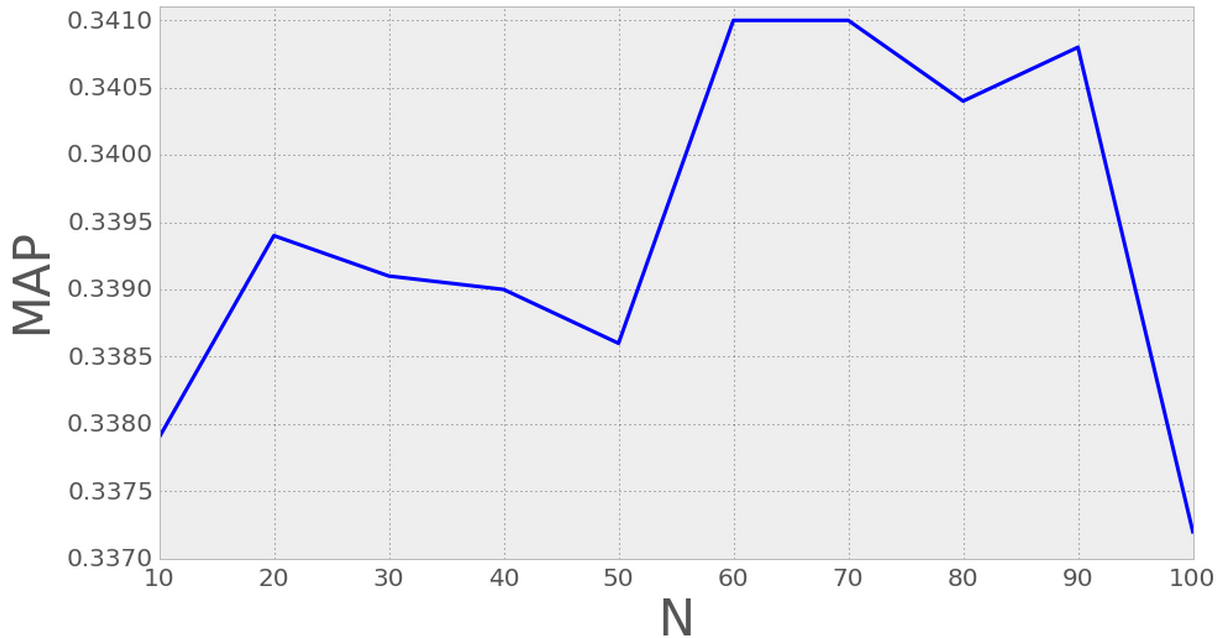
\includegraphics[width=\textwidth]{figures/lab7_N.png}
		\caption[]%
		{{\small Laboratorio 7 (\textsc{hits}), al variare di $N$.}}    
		\label{fig:lab7_Nd}
	\end{subfigure}
        \caption[ The average and standard deviation of claboratorioritical parameters ]
        {\small MAP al variare di alcuni parametri di configurazione della funzione di reperimento, per i diversi laboratori.} 
        \label{fig:map_all}
\end{figure*}
Come si pu\`o vedere da Figura \ref{fig:lab4_R} e Figura \ref{fig:lab6_Nd}, il \textsc{rf pseudo} e l'\textsc{lsa} peggiorano il valore della MAP al crescere del numero di documenti considerati rilevanti, e del numero di documenti da riordinare, rispettivamente. Ci\`o significa che dopo il primo passaggio di \textsc{bm25} l'ordine dei documenti \`e gi\`a preciso, e che l'effetto dello pseudo \textsc{rf} e di \textsc{lsa} \`e quello di alterare tale ordine, peggiorando l'efficacia del reperimento. In Figura \ref{fig:lab5_a} vediamo che $\alpha$ il parametro che regola l'influenza di \textsc{pagerank} sull'ordine dei documenti, ha un effetto molto negativo per valori piccoli, mentre migliora per valori pi\`u alti. Infine in Figura \ref{fig:lab7_Nd} vediamo che il reperimento che si avvale di \textsc{hits} ha un massimo per $N=60$, il che significa che se andiamo ad espandere un insieme radice di 60 elementi otteniamo in media la miglior MAP dopo il riordinamento.

Figura \ref{fig:map_hist} mostra le MAP dei vari metodi di reperimento a partire dalla configurazione \textsc{baseline} di \textsc{bm25} (laboratorio 3), scegliendo la miglior combinazione di parametri per ciascuno di essi. 
\begin{figure}[htpb]
	\begin{center}
		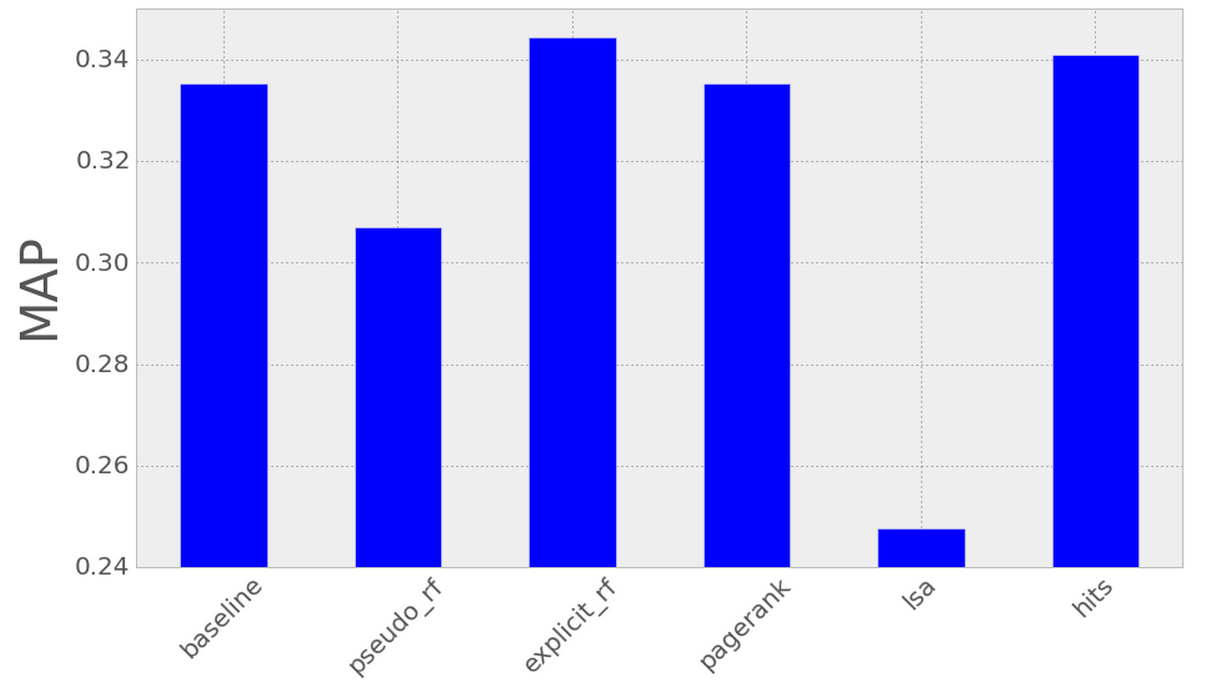
\includegraphics[width=0.75\textwidth]{figures/hist_map.png}
		\caption{MAP per i vari metodi di reperimento, a partire dai parametri di \textsc{bm25} della \textsc{baseline}.}
		\label{fig:map_hist}
	\end{center}
\end{figure}
Tabella \ref{tab:map} riporta i parametri usati per ogni funzione di reperimento e la relativa MAP ottenuta.
\begin{table}[htpb]
	\begin{center}
		\begin{tabular}{|c|c|c|}
			\hline
			metodo & parametri & MAP \\
			\hline
			\textsc{baseline} & - & $0.3354$ \\
			\textsc{rf esplicito} & - & $0.3445$ \\
			\textsc{rf pseudo} & $R=10$ & $0.3071$ \\
			\textsc{pagerank} & $\alpha=1.0$ & $0.3354$ \\
			\textsc{lsa} & $N=10, m=2$ & $0.2477$ \\
			\textsc{hits} & $\alpha=1.0, \beta=0.1, \gamma=0.1, N=60$ & $0.3410$ \\
			\hline
		\end{tabular}
	\end{center}
	\caption{Dettaglio dei parametri usati per le varie funzioni di reperimento e della relativa map. I parametri di \textsc{bm25} per ogni metodo sono quelli della \textsc{baseline} $k_1 = 0.0253, b = 0.0221$.}
	\label{tab:map}
\end{table}

Dai risultati riportati si pu\`o notare che gli unici metodi che hanno portato un miglioramento in termini di MAP rispetto alla \textsc{baseline}, sono l'uso del \textsc{rf esplicito}, e quello di \textsc{hits}. Il notevole peggioramento portato da \textsc{lsa} pu\`o essere spiegato dalla rappresentazione dei documenti nello spazio vettoriale, infatti essi contentendo molto pochi termini in media, sono vettori con molti elementi a zero. Ci\`o significa che nel nostro contesto, dopo la riduzione dimensionale, le similarit\`a tra i vettori non sono significative. In particolare la capacit\`a di \textsc{lsa} di mitigare il problema di sinonimia non \`e efficace, probabilmente perch\`e la collezione \`e piuttosto ristretta. Il riordinamento quindi sposta alcuni documenti rilevanti dalla cima della classifica verso il fondo. Per il \textsc{pagerank} invece possiamo vedere che sebbene esso non abbia portato un miglioramento partendo dai parametri della \textsc{baseline} (per $\alpha = 1$ il contributo di \textsc{pagerank} viene completamente ignorato nel reperimento), utilizzando $\alpha$ come parametro da ottimizzare, tale metodo pu\`o portare un leggero miglioramento della precisione, come riportato in Tabella \ref{tab:es}. In particolare, osservando che anche \textsc{hits} ha portato un aumento della MAP in questi termini, possiamo affermare che l'analisi del grafo delle citazioni porta informazione utile alla rilevanza.

\subsection{Efficienza}
\label{sec:efficienza}
Figura \ref{fig:efficiency} riporta i tempi di esecuzione delle varie funzioni di reperimento, per l'intero set di queries fornite. I parametri utilizzati sono quelli riportati in Tabella \ref{tab:map}. Per ogni metodo si presume che l'indicizzazione sia gi\`a avvenuta, e inoltre tutte le misure calcolabili offline (a tempo di indicizzazione) siano gi\`a state computate (e.g.: il dizionario, le lunghezze dei documenti, la DTM, il valore di pagerank). Come si pu\`o vedere, in particolare grazie alla \textit{vectorization} usata per effettuare il calcolo di \textsc{bm25}, il tempo di esecuzione del reperimento \textsc{baseline} \`e molto breve, poco pi\`u di un secondo. 
\begin{figure}[htpb]
	\begin{center}
		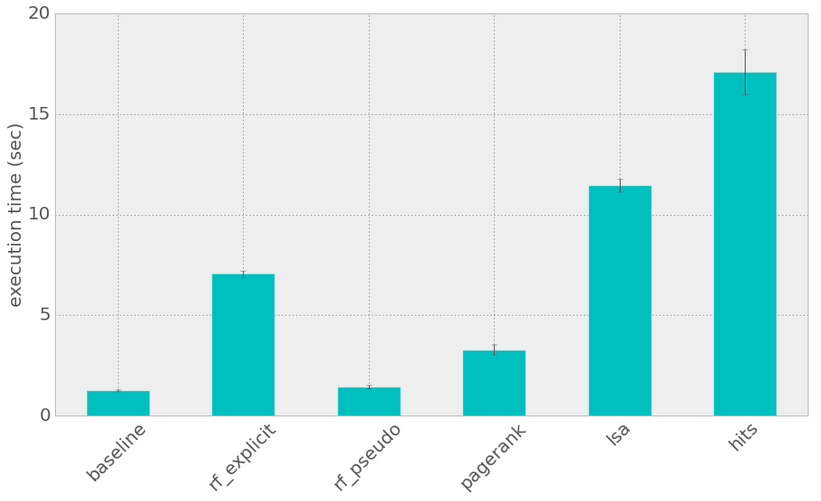
\includegraphics[width=0.75\textwidth]{figures/efficiency.png}
		\caption{Tempo di esecuzione (secondi) e relativa standard deviation per le varie funzioni di reperimento sull'intero set di queries. Media su 20 run. Le run vengono eseguite su thread singolo.}
		\label{fig:efficiency}
	\end{center}
\end{figure}
Gli altri metodi di reperimento sono invece pi\`u impegnativi. In particolare, i metodi \textsc{lsa} e \textsc{hits} sono molto lenti, nel primo caso per la costosa decomposizione \textsc{svd} e il calcolo delle cosine similarity, nel secondo per l'espansione del grafo radice. Gli altri metodi hanno comunque dell'overhead dovuto ai tempi di lettura dei dati addizionali e al riordinamento della lista di documenti.

Tali risultati sono da considerarsi indicativi, in quanto non sono state usate regole vincolanti sul codice volte a garantire l'efficienza. Inoltre la dimensione della collezione  utilizzata ci ha permesso di effettuare maggior parte delle computazioni utilizzando matrici. Tale vantaggio non \`e applicabile al crescere del corpo di documenti.

%Questo paragrafo presenta e discute i risultati sperimentali. Si dovranno
%scegliere tre \textit{run} al massimo per ciascuno dei metodi illustrati nei
%paragrafi \ref{sec:metodi-di-reper}, \ref{sec:relevance-feedback},
%\ref{sec:pagerank}, \ref{sec:lsa} e \ref{sec:hits}.  
%
%Si dovranno confrontare le misure di efficacia (ad esempio, \textit{Mean Average
%  Precision}, MAP) mediante illustrazioni anche grafiche. Un'analisi della
%significativit\`a statistica delle differenze tra i valori di MAP sarebbe
%opportuna.
%
%Un confronto particolare dovr\`a essere fatto tra la \textit{baseline} del
%paragrafo \ref{sec:metodi-di-reper} e i metodi dei paragrafi successivi.
%
%La parte preziosa di questo paragrafo \`e la discussione dei risultati. Si
%dovr\`a dare un'interpretazione ragionata, chiara ed esaustiva delle ipotesi per
%cui sono state osservate o meno le differenze tra i valori di MAP. 

